% vim:textwidth=70
\chapter{可自管理的分布式应用管理工具}
\label{chap:selfman}

%问题,相关工作,创新点,基本\textbf{方法},实验

%问题提出:管理系统是一个分布式应用,同样需要管理
%
%目前的办法:集中部署启动管理系统到各个机器上,并集中式探测、维护(需要
%确认,或者说确定目前方法的缺陷)
%
%集中式的:plush,smartfrog,app-manager,globus,cfengine,还有
%
%plush, app-manager, smartfrog, cfengine, globus, amazon ec2
%
%==========
%为什么要管理管理系统:部署是必须的。更新是必须的。监测呢?可以用cron。
%
%ec2上可以用预装了plush的AMI
%
%攻击点:部署和更新也不经常有,监测死活可以用cron,管理节点死了几个也没事,
%早晚会发现,在那么大规模上,节点多几个少几个没太大问题。
%
%目前管理管理系统的办法有什么不足:
%
%一个可能得点:象self-host文章说的那样,说app希望可以改变运行的节点
%===========
%
%基本方法:节点相互探测对方状态,依据探测的结果,进行相应的管理步骤,实现
%
%系统的自管理。
%
%挑战:可扩展,鲁棒稳定,支持安全的自动认证,扩展管理能力(?)
%
%设计理念:简单、无状态(microreboot?)

\section{本章引论}

分布式系统~\cite{Ghemawat2003,DeCandia2007}是当今internet服务~
\cite{google, amazon?}的关键组成部分。随着普通计算机硬件成本越来越低,
搭建一个规模成百上千的分布式计算平台是很普通的事情。一些常见的分布式计
算平台包括Planet-Lab~\cite{Bavier2004}, Amazon
EC2~\cite{Garfinkel2007} and Teragrid~\cite{Catlett2002}。这些计算平台
可以提供大容量的存贮能力和巨大的计算能力,因此,设计良好的应用可以充
分利用这些资源来提升自己的性能。

随着分布式应用的规模越来越大,有效的管理它们越来越有挑战性。分布式应用
管理系统就是用来简化部署和维护分布式应用的系统。为了有效的完成管理
任务,管理系统也被设计为一个复杂的分布式系统。一个管理系统包括运行在不
同机器上的若干“节点\footnote{对于采用集中式算法的管理系统,节点就是所
谓的客户端}”。这些管理节点间形成一个覆盖网络,节点相互合作来部署分布
式应用。当分布式应用被部署并启动以后,这些管理节点可以监测并维护运行在
同一机器内的应用节点。管理员可以通过管理系统查询应用的状态,或者按照需
求向应用发送控制命令。

我们注意到,由于管理系统实际上也是一个分布式系统,或者说分布式应用,这
带来了一个重要的问题:管理系统也需要被管理。首先,需要把管理节点部署到
一组机器上去,其次,\note{这里需要想想怎么说}

在本文中,我们提出了可自管理的覆盖网络(SMON, Self-Managed Overlay
Network)。SMON是一个新颖的分布式应用管理系统,它具有内建自管理能力,
包括自我部署、自我更新和自我恢复能力。因而,它有效的解决了分布式管理系
统也需要管理的问题。SMON包括分布在一组机器上的管理节点,这些节点相互探
测对方的状态,依据探测的结果,自动执行自我管理任务,包括安装新的SMON管
理节点、更新SMON管理节点至新的版本,或者恢复失败的SMON管理节点。这样,
从整体来看,SMON具有了自我管理的能力。

作为一个分布式应用管理系统,SMON提供了一组基本的管理语意。\note{应用管
理,拓展管理能力。}

设计SMON需要解决一下几个挑战性问题。

首先,SMON需要有良好的可扩展性。其次,为了让SMON节点能够自动在远程机器
上安装新的SMON节点,或者恢复失败的节点,需要有安全机制使SMON节点能够自
动与远程机器认证并登陆,同时保护用户的认证信息(例如私钥)不会被泄露。
最后,SMON的管理能力应该是能够被拓展的。

SMON的设计分别处理了上面几个问题,叙述如下。对第一个问题,SMON的节点构
成一个无结构的覆盖网络,节点间使用epidemic算法相互探测,并执行管理任务。
epidemic算法保证了SMON系统具有良好的扩展性($O(\log N)$),同时
epidemic算法也带来了额外的好处,首先它易于实现,其次,它使得SMON系统很
鲁棒,可以很好的应对网络分割(network partition)错误。对于第二个问题,
我们引入了一个认证代理来帮助SMON节点与远程机器认证。认证代理保存着认证
过程中需要的认证信息(例如私钥),它并不将认证信息泄露给任何SMON节点,
或其它外部对象。简单的说,SMON节点会将认证过程中收到的挑战密文(
challenge)转发给认证代理,并将认证代理回复的应答密文(response)发送
给远程机器,从而完成了自动认证的过程。对于第三个问题,我们可以在SMON上
面部署新的管理系统来扩展系统整体的管理能力。这样,任何部署在SMON之上的
分布式应用,都具有了自管理的能力。

本章接来下的部分安排如下:\note{xxx}

\section{设计}

\begin{figure}
  \centering
  \begin{minipage}{0.8\linewidth}
    \centering
    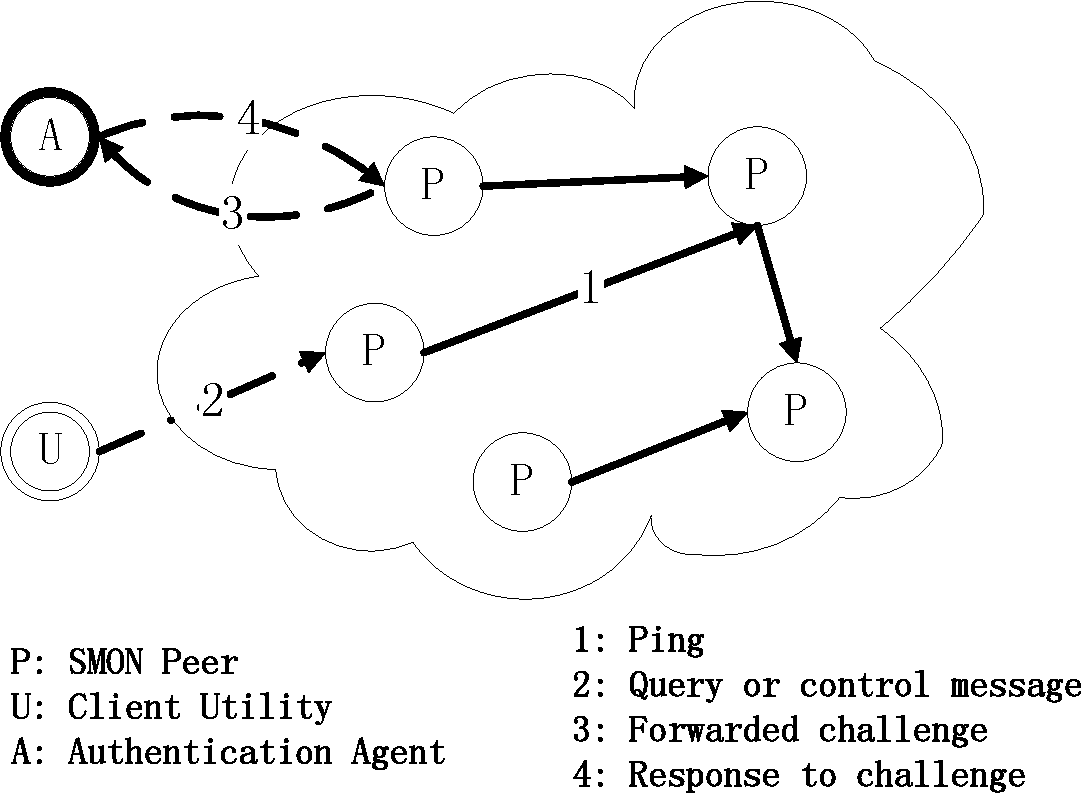
\includegraphics[width=3.0in]{smon_arch}
    \caption[SMON系统结构]{SMON系统结构。SMON系统由三部分构成,
    SMON管理节点、认证代理和
    客户端工具。SMON节点构成SMON系统的主要部分,认证代理协助SMON节点与远程
    机器认证,使用者通过客户端工具完成管理任务。}
    \label{fig:smon_arch}
  \end{minipage}
\end{figure}

SMON系统的体系结构如图~\ref{fig:smon_arch}所示,包含了三个部分:SMON节
点,认证代理和客户端工具。

SMON管理节点运行在分布式平台的一组机器上,每个节点都维护着完整的机器列
表,这个列表也称作是SMON节点的邻居列表。SMON节点相互探测并相互维护。
SMON节点定期从从邻居列表中选择一个节点,向它发一个ping消息,如果超时没
有收到回复的pong消息,那么这个SMON节点会试图向远程机器安装新的SMON节点,
如果远程机器已经安装有SMON节点,那么它将会试图恢复失败的SMON节点运行。
每个SMON节点都保存着自身的版本号,在用ping-pong消息相互探测过程中,会
顺便交换相互的版本号,低版本的SMON节点会将自身升级至高版本。

认证代理持有与分布式平台上的机器认证所需的认证信息(例如私钥)。当
SMON节点在远程机器上部署新的SMON节点,或者恢复失败的SMON节点时,需要首
先与远程机器认证并登陆,这一过程需要认证代理的协助。

用户使用客户端工具来管理一组分布式应用,这其中包括其它分布式管理系统。
通过这个办法,我们可以不断扩充SMON的管理能力。\note{这个说法需要斟酌。}

\subsection{SMON的自我管理}

我们分别描述SMON自我管理的三个方面:自我部署,自我更新和自我恢复。

\subsubsection*{自我部署}

% 一些啰嗦的表达方式:
% SMON可以自动部署至一组节点,一组分布式节点
% 相互探测,相互维护
% ping -> liveness

SMON可以自动将自己部署至分布式平台的一组目标机器上去。在最初状态时,所
有的目标机器上都没有被部署运行SMON节点。用户需要手动部署并启动一个SMON
节点。这个SMON节点会在邻居列表中随机选取一个机器,并在它上面部署第二个
SMON节点。新的SMON节点同样会在别的机器上部署SMON节点。当越来越多的SMON
节点被部署,自我部署过程会以幂指数速度增长。可以证明,以概率1,
所有可以连接的机器上都会被部署SMON节点~\cite{Eugster2004}。

详细来说,节点$P$会定期选择邻居列表里的一个机器$M$,并向它上发送SMON节
点探测消息(ping)。如果超时没有收到回应的pong消息,$P$就会在$M$上远程
部署一份SMON节点。它首先在认证代理的协助下(在\ref{subsec:security}节
中描述)认证并登陆进$M$,向$M$远程拷贝一份SMON的安装程序,并远程启动安
装程序。启动的安装程序首先检查自己的完整性(使用checksum校验和),以防
传输过程中产生错误,然后它会安装并启动SMON节点。

在上述过程运行的任何时刻,都有可能因为外界因素而产生错误(例如连接中断,
机器崩溃等)。如果有错误发生,$P$会直接放弃这次远程部署的任务。
epidemic算法能够保证,在未来,$M$会被另外一个SMON节点$P'$选中并部署
SMON节点。

自我部署过程中存在着竞争情形(race condition)。因为采用了epidemic算法,
多个SMON节点可能同时试图向同一个机器$M$部署SMON节点。这个问题不需要
SMON节点间直接协调便可以解决。不同SMON节点会将安装程序远程复制到$M$上的
不同目录,相互不会覆盖。如果有多份安装程序被同时启动,它们会使用操作系
统提供的同步机制(例如lock file),保证只有一份安装程序能够运行。因此,
只有第一个运行的安装程序能够完成安装。在解决这个竞争情形的过程中,引入
了一定的额外负载,会有多份安装程序被拷贝至同一台机器。这会浪费一部分存
储资源和网络带宽。经过实验测试,可以看出额外负载的数量在多大数机器上是
很小的。同时考虑到安装程序很小,只有122KB,因此可以认为额外负载的影响
不大。

自我部署过程何时结束是难以严格确定的。理想情况是,当所有目标节点上都被
部署并运行着SMON节点时,自我部署过程就可以称为结束了。但是,在分布式环
境下,某些节点可能会发生错误,或者不可连接,所以,实际情况下自我部署过
程很难达到理想情况。即使一个机器已经被部署了SMON节点,也有可能因为机器
或者网络错误的原因,造成某些SMON节点被关闭或者不可连接。因此,为了应对
分布式环境频繁发生的异常错误,每个SMON节点需要不断的监控其它节点。自我
部署何时结束是一个需要用户定义的问题。用户可以查询有多少机器已经部署且
运行着SMON节点,根据需要决定自我部署是否结束。

\subsubsection*{自我更新}

SMON可以将自己自动更新至新的新的版本。这个更新过程是在线进行的,用户不
需要因为更新而停止整个SMON系统。

每个SMON节点都有版本号,版本号被持久保存在每个SMON节点的配置文件中。
SMON节点会以epidemic方式交换相互的版本号。当发现相互的版本不同,版本低
的SMON节点会自动从高版本SMON节点那里获取新的安装程序,将自己更新至高版
本。为了把整个SMON系统更新至新版本,用户只需要更新一个SMON节点,整个
SMON系统会逐渐收敛至一个最终的版本。用户使用~\ref{subsec:client}节中描
述的客户端工具更新任何一个SMON节点。

存在着多个SMON节点向同一个版本SMON节点请求安装程序的可能,为了防止
瞬间拥挤(flash crowd)的冲击,节点会限制同时请求安装程序的数量。

\subsubsection*{自我恢复}

SMON系统可能遇到两种分布式环境中产生的错误:机器失败和网络分割。当一个
机器失败时,它上面运行的SMON节点也同时会被停止。SMON节点会尝试重新启动
失败的SMON节点,因此一旦失败的机器恢复,它上面的SMON节点会被重新启动。
同时启动多份SMON节点的实例是安全的,使用操作系统的同步机制,这等同于只
启动一个SMON实例。

网络分割也很容易应对。当网络分割发生时,SMON系统被分割为多个部分,每个
部分将会成为一个独立的小SMON系统,它们的状态,例如运行的SMON节点版本,
都将在各个部分内逐渐达成一致。当被分割的部分重新连接上时,不同部分的
节点会重新相互联系,从而整个系统的状态逐渐收敛。

\subsubsection*{自我管理小结}

将上述三个部分合并起来,就构成了SMON自我管理的内容。SMON节点通过相互探
测并执行相应的管理任务来达到整个SMON系统自我管理的目标。有两点值得说明。
第一、作为一个优化,SMON间使用ping-pong消息探测时,会顺便交换
(piggyback)它们的版本号。第二、如果节点$A$认为节点$B$失败,可能有两
个原因,或者$B$没有运行,或者$B$所在机器没有部署SMON节点。$A$会首先判
断远程机器上是否部署了SMON,并采取相应的步骤。

\subsubsection*{禁止、启动自我管理功能}

SMON的自我管理功能应该是能够被显式的禁止或者启动的。考虑如下场景:某个
研究人员使用SMON部署了一个分布式系统原型,在进行一些实验后,他决定停止
部署的分布式系统和SMON。如果SMON的自我管理功能没有被禁止,则整个SMON系
统不能够被停止。任何被用户停止的SMON节点,都很快会被其它SMON节点启动,
除非用户能够在一瞬间停止所有SMON节点,然而这在大规模分布式系统上是不可
能。

我们使用一个布尔变量\texttt{livetag}控制SMON节点的自我管理功能。如果它
的值是假,则节点停止定期探测其它节点的活动,因此整个系统停止了自我管理
的功能。这样,我们就能够逐一停止SMON节点,从而停止整个SMON系统了。

\texttt{livetag}变量有一个关联的版本号,每个SMON节点维护着变量的一个复
本。两个随机节点会定期交换\texttt{$<$livetag, version$>$}对,并且更新
\texttt{livetag}到最新的版本。需要注意到,节点交换\texttt{livetag}的行
为也是收到\texttt{livetag}值的控制的。当\texttt{livetag}值为假,节点不
会主动要求交换\texttt{$<$livetag, version$>$}对,但是任然会对交换消息
回复,这能够加快更新\texttt{livetag}的速度。

\subsection{安全机制}
\label{subsec:security}

SMON的安全机制需要保证如下两个目标:

\begin{itemize}

  \item 让节点能够自动与其它机器认证并登陆,从而节点能够自动安装新的
  SMON节点,或者远程恢复失败的SMON节点。

  \item 认证并加密SMON节点间的通信,不让系统被恶意利用,被用来部署
  恶意应用,例如botnet~\cite{botnet}。

\end{itemize}

我们首先叙述如何在Planet-Lab上设计达到上述两个目标的安全机制,并解释如
何在其它分布式计算平台上应用这个机制。Planet-Lab使用公钥系统来认证对系
统平台的访问。每个用户使用ssh访问他的slice~\footnote{Planet-Lab分配给
用户的一组分布式资源,表现形式是一组分布式虚拟机。}。用户私钥保存在
自己的机器上,对应的公钥被分发到用户slice的所有虚拟机里。

\begin{figure}
\centering
  \begin{minipage}{0.8\linewidth}
    \centering
    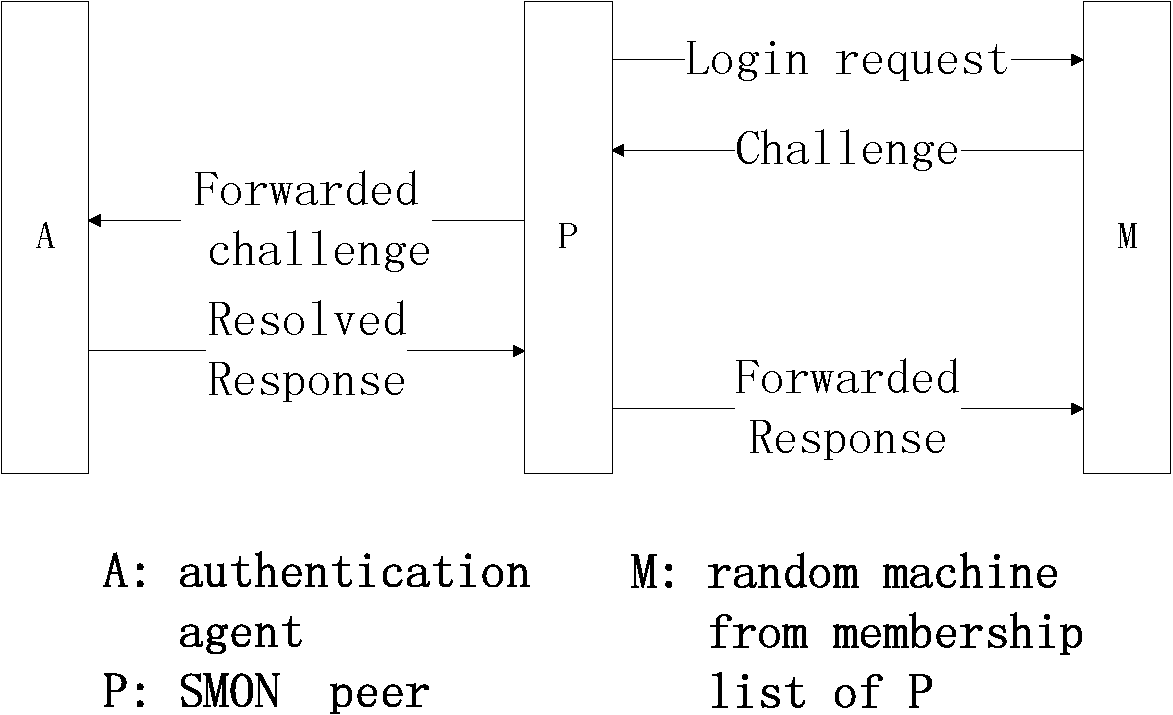
\includegraphics[width=3.0in]{auth}
    \caption{SMON节点在认证代理协助下与远程机器认证并登陆的过程。图显示
    了这一过程中三者的交互过程。}
    \label{fig:auth}
  \end{minipage}
\end{figure}

SMON引入了认证代理来协助节点自动与远程机器认证。认证代理持有用户私钥,
但私钥并不会被泄露。如图~\ref{fig:auth}所示,当SMON节点需要登陆到其它
机器上时,它首先连接远程机器的sshd服务器,并发送登陆请求。sshd服务器会
返回一个认证挑战密文,SMON节点没有用户私钥,无法求解对应的应答密文,它
会直接将挑战密文转发给认证代理,认证代理使用用户私钥求解得到应答密文,
并告诉SMON节点。SMON节点再将应答密文发送给sshd服务器。这样,SMON节点能
够登陆到用户slice内的任何一台机器上,并且用户私钥并未被泄露。

我们使用一个对称密钥$K_E$来认证和加密SMON节点之间、SMON节点和认证代理
之间的通信。$K_E$在SMON节点部署时一同被部署到各个机器上。由于部署的过
程中,通信是加密的,因此$K_E$不会被泄露。$K_E$也是可以安全保存在slice
内的机器上的,因为slice的虚拟机之间被很好的相互隔离。

用户应仔细评估并选择认证代理运行的机器,保证用户私钥的安全。认证代理不
必运行在用户slice内的某个机器上。如果SMON被部署的规模非常大,可以考虑
运行多份认证代理,提高认证的性能,同时有效的应对网络分割错误。SMON节点
可以在DNS服务器协助下~\cite{dns_akamai},将选择离自己最近的认证代理。

上面叙述的安全机制可以推广应用到其它分布式平台上,如果分布式平台满足下
面的两个假设:

\begin{itemize}
  \item

  \item
\end{itemize}


\subsection{客户端工具}
\label{subsec:client}

\section{应用方式}
plush

d3s

scalpel

\section{性能评价}

\section{相关工作}

\section{本章小节}
